\documentclass{article}
%\usepackage{graphics,psfrag}
\usepackage{dkthesis,calc,array,amsmath,tabularx,program,graphicx,psfrag,becs}
\begin{document}
Some text.
\begin{figure}
\psfrag{PShello1}{Test}
\begin{center}

\includegraphics{METHODS/test.eps}
\end{center}
\caption{A figure\label{fig:test}}
\end{figure}
And some more text.
\begin{figure}
\begin{center}
\psfrag{PShello1}{$Z_1 \cap Z_2, \forwardproj{Z_1}, Z_2[h_1:=0]$}
\psfrag{h1}{$h_1$}
\psfrag{h2}{$h_2$}
\psfrag{Z1}{$Z_1$}
\psfrag{Z2}{$Z_2$}
\psfrag{Z1iiZ2}{$Z_1 \cap Z_2$}
%\epsfxsize=.8\linewidth
%\epsffile{METHODS/poly.eps}
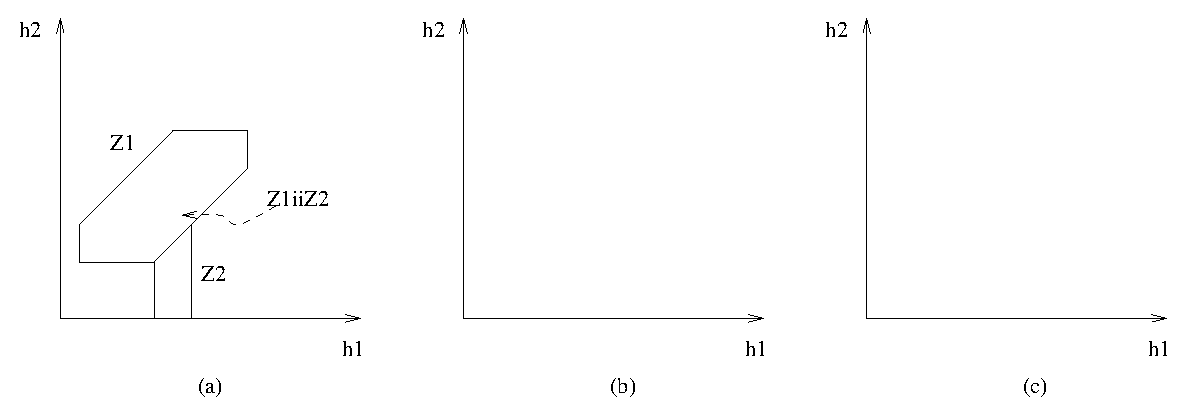
\includegraphics{METHODS/poly.eps}
\end{center}
\caption{Polyhedra: $Z_1 \cap Z_2, \forwardproj{Z_1}, Z_2[h_1:=0]$}
\end{figure}
And another figure.
\end{document}